\documentclass[letterpaper,11pt]{article}

\usepackage{listings}
\usepackage{color}

\definecolor{dkgreen}{rgb}{0,0.6,0}
\definecolor{gray}{rgb}{0.5,0.5,0.5}
\definecolor{mauve}{rgb}{0.58,0,0.82}

\lstset{frame=tb,
  language=Python,
  aboveskip=3mm,
  belowskip=3mm,
  showstringspaces=false,
  columns=flexible,
  basicstyle={\small\ttfamily},
  numbers=none,
  numberstyle=\tiny\color{gray},
  keywordstyle=\color{blue},
  commentstyle=\color{dkgreen},
  stringstyle=\color{mauve},
  breaklines=true,
  breakatwhitespace=true,
  tabsize=3
}

\usepackage{setspace}
\usepackage{graphicx}
\usepackage{indentfirst}
\usepackage{bm}    %for textbf
\usepackage{amsmath}
\usepackage{amsfonts}   %for mathbb
\allowdisplaybreaks[4]  %from {amsmath}
\newcommand{\independent}{\rotatebox[origin=c]{90}{$\models$}}  %from {graphicx}
\usepackage{geometry}
\geometry{letterpaper, scale=0.8}  %from {geometry}
\author{Yuan Yin A20447290}
\title{MATH 584 Homework 3}
\begin{document}\large
\maketitle
\begin{spacing}{1.2}  %from {setspace}

Before the writte up, I first claim some settings different from the problem statement. Due to the large time of running, I only use the first 2 assets to do problem 1 and 5 assets to do problem 2. And also for transaction costs I only do with Transaction cost $\lambda = 0$ case.

\section*{Problem 1}
\subsection*{(a)}
For this question, I use first 2 assets and test the strategy using T-costs $\lambda = 0$. I plot the relative PnL and absolute PnL process and save all PnL values in ``absolute\_PnL1.csv'' and ``relative\_PnL1.csv'' files.

The Sharpe Ratio for absolute PnL is $-0.028858250792814597$, and for relative PnL is too small to show.

The plot is as follows:
\begin{figure}[h] %h for head or t for top
\centering
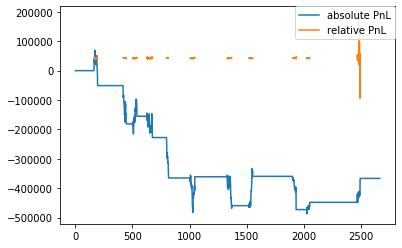
\includegraphics[scale=0.5]{1a pnl.png}
\caption{PnL process for asset 1}
\label{fig:label}
\end{figure}

\subsection*{(b)}
For this question, I use first 2 assets and test the strategy using T-costs $\lambda = 0$. I plot the relative PnL and absolute PnL process and save all PnL values in ``absolute\_PnL1b.csv'' and ``relative\_PnL1b.csv'' files.

The Sharpe Ratio for absolute PnL is $-0.018348849866976644$, and for relative PnL is too small to show.

The plot is as follows:
\begin{figure}[h] %h for head or t for top
\centering
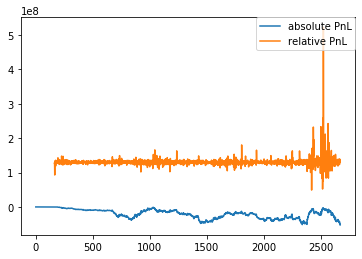
\includegraphics[scale=0.5]{1b pnl.png}
\caption{PnL process for asset 1}
\label{fig:label}
\end{figure}

\subsection*{(c)}
For this question, I use first 5 assets and test the strategy using T-costs $\lambda = 0$. I plot the relative PnL and absolute PnL process and save all PnL values in ``absolute\_PnL1b.csv'' and ``relative\_PnL1b.csv'' files.

The Sharpe Ratio for absolute PnL is $0.060693118141089165$, and for relative PnL is too small to show.

The plot is as follows:
\begin{figure}[h] %h for head or t for top
\centering
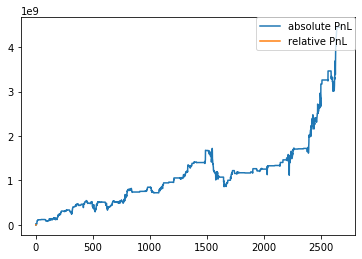
\includegraphics[scale=0.5]{2 pnl.png}
\caption{PnL process for asset 1}
\label{fig:label}
\end{figure}

\end{spacing}
\end{document}